\documentclass[12pt]{article}

\usepackage{graphicx}
\usepackage[cm]{fullpage}
\usepackage{fixltx2e}
\usepackage{hyperref}
\usepackage{mathtools}
\usepackage{amsmath}
\usepackage{enumerate}
\usepackage{listings}
\usepackage{color}
\usepackage{framed}
\usepackage{eurosym}
\usepackage{changepage}
\setcounter{secnumdepth}{3}
\renewcommand\thesection{\arabic{section}}
\renewcommand\thesubsection{\thesection.\arabic{subsection}}
\definecolor{mygreen}{rgb}{0,0.6,0}
\definecolor{mygray}{rgb}{0.7,0.7,0.7}
\setlength{\oddsidemargin}{0.0in}
\setlength{\evensidemargin}{0.0in}
\setlength{\topmargin}{-0.25in}
\setlength{\headheight}{0in}
\setlength{\headsep}{0in}
\setlength{\textwidth}{6.5in}
\setlength{\textheight}{9.25in}
\setlength{\parindent}{7mm}
\setlength{\parskip}{0mm}
\begin{document}
\raggedright{

%%%%%%%%%%%%%%%%%%%%%%%%%%%%%%%%%%%%%%%%%
% University Assignment Title Page 
% LaTeX Template
% Version 1.0 (27/12/12)
%
% This template has been downloaded from:
% http://www.LaTeXTemplates.com
%
% Original author:
% WikiBooks (http://en.wikibooks.org/wiki/LaTeX/Title_Creation)
%
% License:
% CC BY-NC-SA 3.0 (http://creativecommons.org/licenses/by-nc-sa/3.0/)
%%%%%%%%%%%%%%%%%%%%%%%%%%%%%%%%%%%%%%%%%

\begin{titlepage}

\newcommand{\HRule}{\rule{\linewidth}{0.5mm}} % Defines a new command for the horizontal lines, change thickness here

\center % Center everything on the page
 
%----------------------------------------------------------------------------------------
%	HEADING SECTIONS
%----------------------------------------------------------------------------------------

\textsc{\LARGE University of California, Davis}\\[1.5cm] % Name of your university/college
\textsc{\Large ECS 158}\\[0.5cm] % Major heading such as course name
\textsc{\large Programming on Parallel Architectures}\\[0.5cm] % Minor heading such as course title

%----------------------------------------------------------------------------------------
%	TITLE SECTION
%----------------------------------------------------------------------------------------

\HRule \\[0.4cm]
{ \huge \bfseries Parallelization of R's combn() Function}\\[0.4cm] % Title of your document
\HRule \\[1.5cm]
 
%----------------------------------------------------------------------------------------
%	AUTHOR SECTION
%----------------------------------------------------------------------------------------

\begin{minipage}{0.4\textwidth}
\begin{flushleft} \large
\emph{Authors:}\\
Trisha \textsc{Funtanilla}\\ % Your name
Syeda \textsc{Inamdar}\\ % Your name
Eva \textsc{Li}\\ % Your name
Jennifer \textsc{Wong}\\ % Your name
\end{flushleft}
\end{minipage}
~
\begin{minipage}{0.4\textwidth}
\begin{flushright} \large
\emph{Professor:} \\
Norm \textsc{Matloff} % Supervisor's Name
\end{flushright}
\end{minipage}\\[4cm]

% If you don't want a supervisor, uncomment the two lines below and remove the section above
%\Large \emph{Author:}\\
%John \textsc{Smith}\\[3cm] % Your name

%----------------------------------------------------------------------------------------
%	DATE SECTION
%----------------------------------------------------------------------------------------

{\large \today}\\[3cm] % Date, change the \today to a set date if you want to be precise

%----------------------------------------------------------------------------------------
%	LOGO SECTION
%----------------------------------------------------------------------------------------

%\includegraphics{Logo}\\[1cm] % Include a department/university logo - this will require the graphicx package
 
%----------------------------------------------------------------------------------------

\vfill % Fill the rest of the page with whitespace

\end{titlepage}

\tableofcontents

\newpage

%------------------- Body----------------------%

\section{Objective}
Choose some function \textbf{\texttt{g()}} in R, either built-in to base R or in a CRAN package, to parallelize. Do so in Snow, OpenMP and CUDA (or substitute Thrust for either CUDA or OpenMP, but not both), and run timing tests.

\section{Function}
We chose to parallelize the function \texttt{combn()} from the ``combinat" package in CRAN.
\subsection{Description}
Taken from the official documentation:\cite{crandoc}\\
\null
\begin{adjustwidth}{2em}{0pt}
``Generate all combinations of the elements of x taken m at a time. If x is a positive integer, returns
all combinations of the elements of seq(x) taken m at a time. If argument ``fun" is not null, applies
a function given by the argument to each point. If simplify is FALSE, returns a list; else returns a
vector or an array. ``..." are passed unchanged to function given by argument fun, if any.''
\end{adjustwidth}

\subsection{Why Speedups Are Possible}

We have tried \texttt{combn()}, which has the inputs \texttt{combn(x, m, fun=NULL, simplify=TRUE, ...)}, with different inputs for the vector $x$ and value $m$. We noticed that \texttt{combn()} became quite slow once $x$ had a size numbering around 100 or higher and $m$ around 5 or higher, taking several minutes to compute (but not print) its results. We think that we can achieve speedups by dividing the input $x$ equally among the threads/nodes, and parallelizing the work of creating the output matrix or list. The goal is to speed up the function, which, based on its source code, currently computes combinations serially.    

\section{Parallelization}

\subsection{OpenMP}

The C++ OpenMP program is called through R via .Call() using the Rcpp interface. It accepts the same input arguments as the original function, can handle the same types of valid inputs, and through new optional arguments, also allows the user to decide on a scheduling policy and chunk size.\\
\null
Code highlights:\\
\begin{itemize}
\item Load balancing algorithm \cite{parallelalgorithm} (next section)
\item Avoidance of critical sections and barriers
\end{itemize}
Other notes:
\begin{itemize}
\item Similar to the original function, the OpenMP implementation has a limit on the input/output size. The program terminates if R decides that it cannot allocate enough space for the output.
\end{itemize}

\subsubsection{Load Balancing}
Good load balancing is very critical to our program because for each element $i$ in the input vector $x$, the number of combinations that can be generated with $x_{i}$ is larger than that with $x_{i+1}$. A naive task distribution without proper load balancing could heavily skew the distribution of the workload for each thread. For example, directly assigning an $x_{i}$ for each thread will result in the threads with lower id's generating far more combinations (thus, more work) than threads with higher id's).\\
\null
In order to compensate for the load imbalance, the assignment of tasks to the threads was done in a wrap around manner. Using this method, for the first distribution, each thread will work on the element indexed in the same value as their id (e.g. thread 0 on $x[0]$, thread 1 on $x[1]$, and so on). Then, the following distribution depends on the total number of threads, the id of each thread, and the index of its previous assignment. With $nth$ corresponding to the total number of threads and $me$ corresponding to the thread id, the assignment following the initial distribution is determined using the equation:
\begin{equation}
next\_task = prev\_task + 2 * (nth - me - 1) + 1
\end{equation}
The distribution that will then follow the above depends on the id of each thread the index of the previous task. This next distribution is determined by the equation:
\begin{equation}
next\_task = prev\_task + 2 * me + 1
\end{equation}
The succeeding distributions alternates in using the two equations until the last distribution, which is for $n - m + 1$ or the last $x_{i}$ that can form a combination of size $m$ with the elements succeeding it.\\
\null
In this algorithm, each thread knows which indexes in $x$ to generate combinations for. The threads do not need to communicate with each other, avoiding huge overhead especially for large values of n.

\subsubsection{Chunk Size}
The equations from the section above implicitly defines the chunk size so that each thread gets assigned roughly the same number $x_{i}$'s to work on. It is essentially the number of times task distributions occur in the load balance algorithm, which is roughly $(n-m+1)/nth$.

\subsubsection{Scheduling Policies}
The load balancing algorithm described in Section 3.1.1 implements a static scheduling policy since the threads are assigned specific tasks and only work on the tasks assigned to them. For the purposes of timing comparisons, additional optional arguments \texttt{sched} and \texttt{chunksize} were added to the function in order to test the speed of the program for the other scheduling policies, namely dynamic and guided. If both arguments are not provided (or set as NULL), the program defaults to the static scheduling policy using the load balancing algorithm. If either dynamic or guided is set, the program uses OpenMP's built-in \texttt{schedule} clause to distribute the tasks to the threads. If the chunksize is not provided, the program sets it to the default chunk size of 1.\\
\null

We performed various tests using the three scheduling policies and experimented with different chunk sizes (for dynamic and guided). It was clear that the load balancing algorithm using static scheduling was the fastest. It eliminates the communication overhead of the dynamic and guided scheduling policies since the threads don't have to repeatedly access the task farm for work, and idleness is still reduced because of the way the tasks are distributed among the threads.\\
\null

Hence, the static method is the one compared to the original function in the timinng comparisons.

\subsubsection{Cache and Other Performance Tuning Considerations}
The following performance tuning applies only to the load balancing algorithm described in 3.1.1.

\begin{itemize}
\item Avoiding instances of false sharing: In order to avoid instances of false sharing (and the resulting cache coherence overheads), we avoided having shared data that could be modified by multiple threads. The data frequently accessed and shared by the threads in the program, such as the input and position vectors are read-only data. Hence, cache lines are not invalidated whenever data from these vectors are accessed. The main shared data structure that is modified by all threads is the output matrix \texttt{retmat}, but the threads never have to perform any read on this data.

\item Synchronization overhead: The threads are made to work as independent of each other as possible. The only synchronization occurs implicitly at the end of the \texttt{parallel} pragma.

\item Avoidance of critical sections and barriers

\end{itemize}



\subsubsection{Comparative Analysis}
The following test inputs were used for comparing the speeds of the source code and our OpenMP implementation using 8 threads.\\
\null

\texttt{> system.time(combn(c(1:100), 2))}\\
\texttt{> system.time(combn(c(1:300), 2))}\\
\texttt{> system.time(combn(c(1:100), 3))}\\
\texttt{> system.time(combn(c(1:150), 3))}\\
\texttt{> system.time(combn(c(1:200), 3))}\\
\texttt{> system.time(combn(c(1:300), 3))}\\
\texttt{> system.time(combn(c(1:250), 3))}\\
\null

Here are the total number of combinations generated for each test above:\\
\null
\texttt{> nCm(100, 2, 0.10000000000000002)}\\
\texttt{[1] 4950}\\
\texttt{> nCm(300, 2, 0.10000000000000002)}\\
\texttt{[1] 44850}\\
\texttt{> nCm(100, 3, 0.10000000000000002)}\\
\texttt{[1] 161700}\\
\texttt{> nCm(150, 3, 0.10000000000000002)}\\
\texttt{[1] 551300}\\
\texttt{> nCm(200, 3, 0.10000000000000002)}\\
\texttt{[1] 1313400}\\
\texttt{> nCm(300, 3, 0.10000000000000002)}\\
\texttt{[1] 4455100}\\
\texttt{> nCm(250, 3, 0.10000000000000002)}\\
\texttt{[1] 2573000}\\
\null

The elapsed time recorded for each test is the average of three trials. The OpenMP parallelization massively improved the performance of the function. The improvement becomes increasingly invaluable as the input size increases (e.g. \texttt{nCm(100, 5)}, the OpenMP implementation still manages to produce an output under 5 seconds, while the original function takes several minutes).\\
\null

The following plot illustrates the differences in the speeds of the two implementations.\\
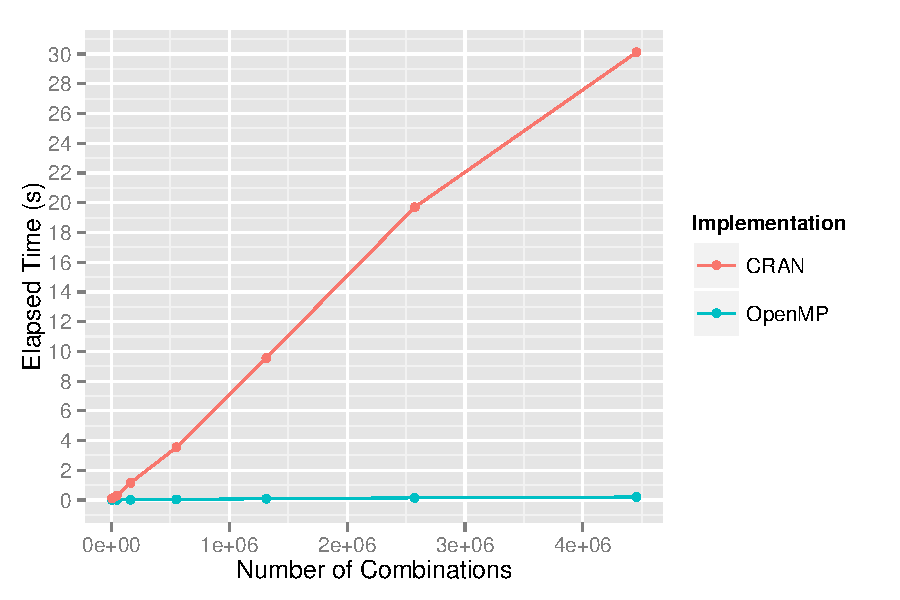
\includegraphics{openmp.pdf}



\subsection{Snow}

The function \texttt{combnsnow()} accepts the same input arguments as the original function \texttt{combn()} from the CRAN package. \texttt{combnsnow()} can also handle the same types of valid inputs (see Section 2.1).\\
\null
Usage:\\
\null

\texttt{combnsnow <- function(cls, x, m, fun = NULL, simplify = TRUE, ...)}\\
\null

where \texttt{cls} is the clusters, \texttt{x} is the input vector of integers and/or characters, \texttt{m} is number of elements per combination
\texttt{fun} is the function to be applied to the resulting output, \texttt{simplify} indicates whether the output must be printed as a matrix (set to \texttt{TRUE}) or as a list (set to \texttt{FALSE}), and \texttt{...} are the parameters for \texttt{fun}.\\

\null
Code highlights:\\
\begin{itemize}
\item Load balancing algorithm implemented in R Snow
\end{itemize}
Other notes:
\begin{itemize}
\item Again, the program terminates if R decides that it cannot allocate enough space for the program to successfully run.
\end{itemize}

\subsubsection{The Issue of Communication Overhead}
After running tests using small inputs, it was observed that parallelization using Snow more often than not took longer than running the CRAN function \texttt{combn()}. This is because of the communication overhead. The communication between the nodes in the cluster took more time than the actual computations in the function. If the jobs sent to the worker nodes are not relatively computationally extensive, the overhead of communicating ends up deteriorating the performance.

\subsubsection{Reducing Network Overhead}
Communication is much slower than computation. There is already communication overhead to setting up clusters. In order to reduce network overhead and improve the performance, the code was written so that the nodes will do long calculations, and the tasks are going to be pre-assigned so that there will be less communications among the nodes as each work on its own tasks. The same load balancing algorithm as in Section 3.1.1 was used to distribute the tasks to each nodes.

\subsubsection{Comparative Analysis}
The same input sizes and function arguments as in Section 3.1.5 were used for testing. For the Snow tests, 8 clusters were used. The following plot illustrates the differences in speeds between the Snow and CRAN implementations:\\
\null

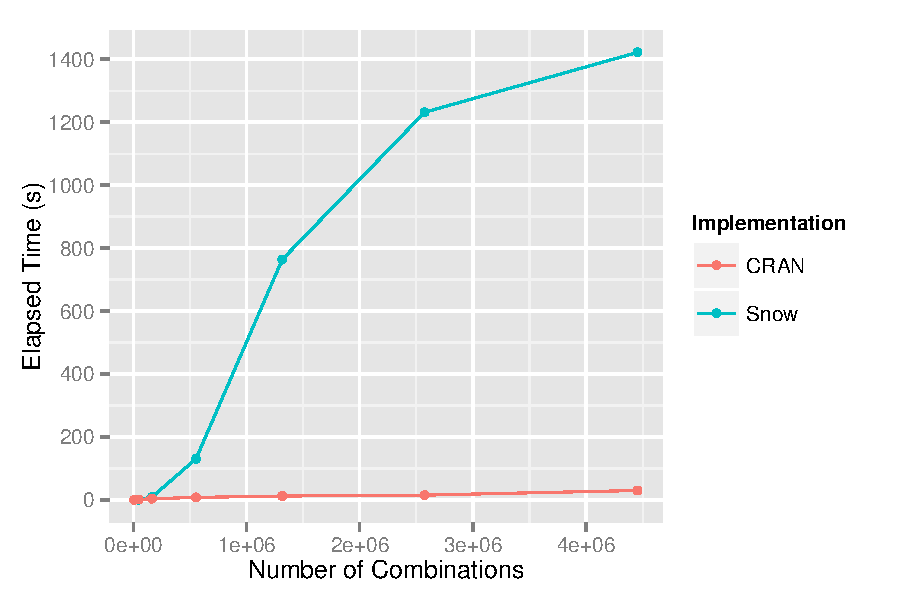
\includegraphics{snow.pdf}\\
\null

Despite our efforts to achieve speedups, the Snow implementation was actually much slower than the serial implementation of \texttt{combn()}. While the load balancing algorithm helped in distributing the tasks, there are other aspects in the code that makes the program slower. For instance, sorting and formatting of the output is not in parallel, which can take a really long time in R when the input size is really big. There is also the inevitable communication overhead due to the use of clusters.








\subsection{Thrust}

\section{Timing Comparisons and Analysis}

The following plot compares all four implementations for various values of \texttt{x} and \texttt{m}. The number of clusters used for Snow and the number of threads used for OpenMP are both 8.\\

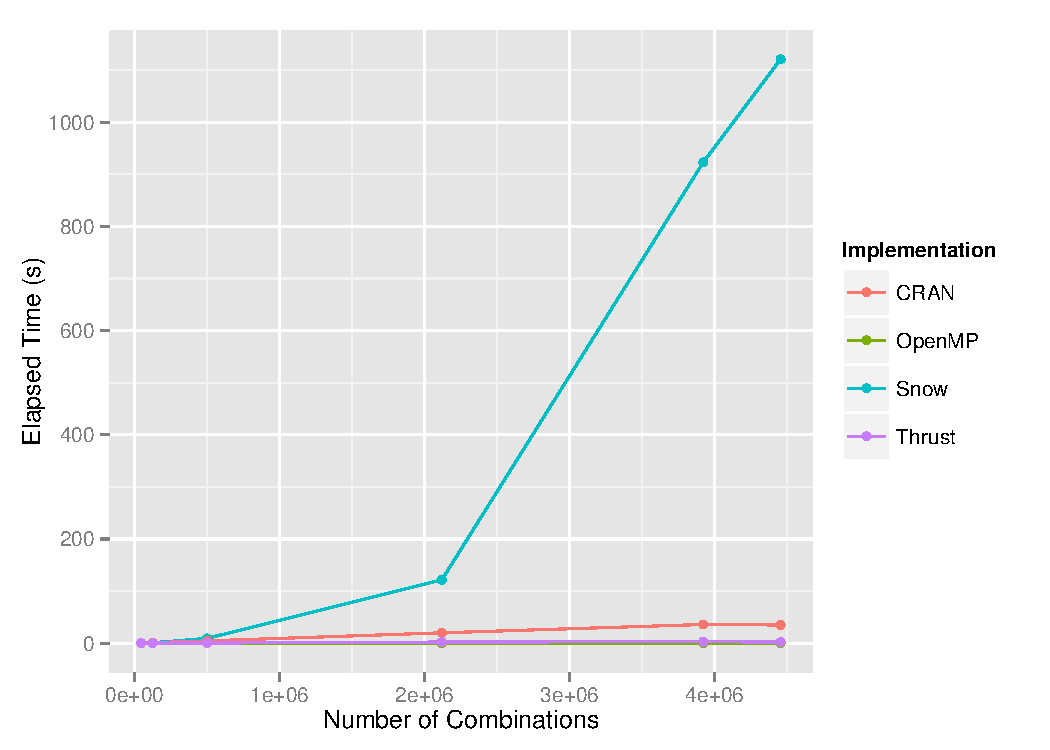
\includegraphics{all.pdf}\\
\null

Clearly, the Snow implementation is simply too slow. By excluding Snow, we can have a closer look on the speeds of the other three implementations:\\

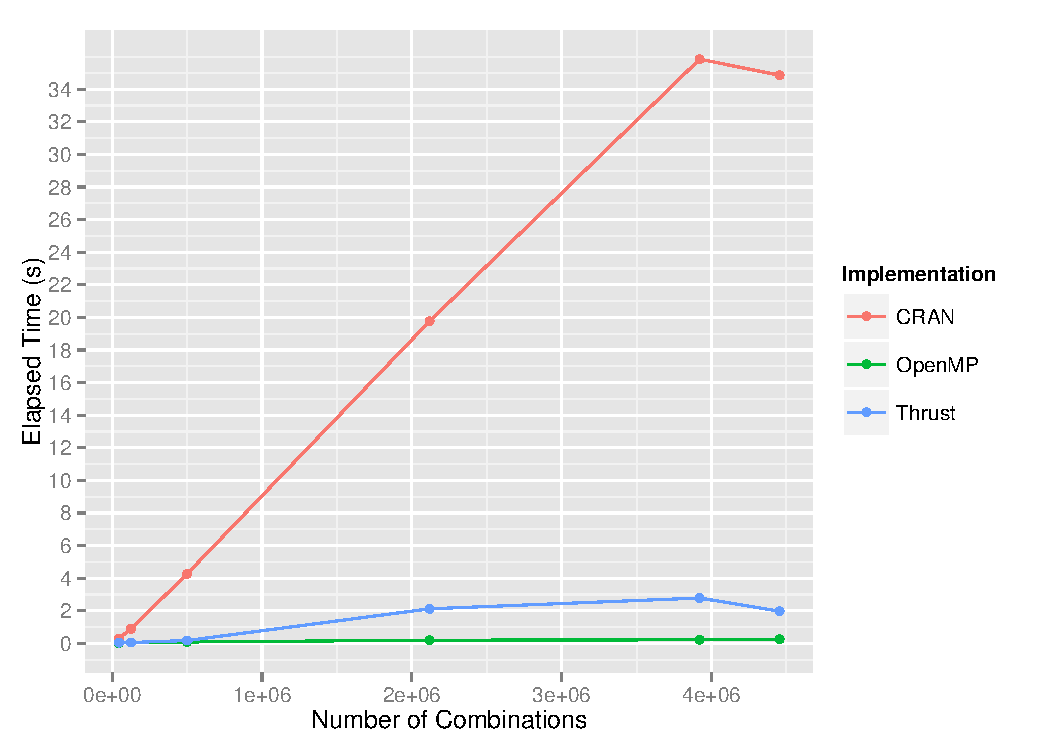
\includegraphics{withoutsnow.pdf}\\
\null

OpenMP and Thrust both massively improved the performance of \texttt{combn()} especially for large inputs. OpenMP was faster, and it also worked for even bigger inputs. We were able to get results for up to 75,287,520 combinations (\texttt{nCm(100, 5)}) in under 5 seconds. The differences in speeds between the OpenMP and Thrust implementations started to become quite significant at around 20,708,500 combinations (\texttt{nCm(500, 3)}). The Thrust program also started to have memory issues past this input size because of the limitations in the memory of the GPU.\\
\null



\section{Conclusions}


%---------------- End of Body ----------------------%


%---------------- Appendix ----------------------%
\newpage

\appendix

\section{Appendix}

{\lstset{
language=R,
backgroundcolor = \color{white},
basicstyle = \scriptsize\ttfamily,
commentstyle=\color{mygreen},
stepnumber=1,
xleftmargin=2em,
framexleftmargin=1.8em,
numbers=left,
numbersep=5pt,
showspaces=false,
showstringspaces=false,
showtabs=false,
frame=single,
rulecolor=\color{black},
tabsize=2,
captionpos=b,
breaklines=true,
breakatwhitespace=false,
keywordstyle=\color{blue},
escapeinside={}
}

% OPENMP R FILE

\begin{lstlisting}
####################################################################################
# R call function for the OpenMP parallelization of combn() from the CRAN
# combinat package: http://cran.r-project.org/web/packages/combinat/index.html

# Function Arguments:
# x <- input vector of integers and/or characters
# m <- number of elements in a combination
# fun <- function to apply to the resulting output
# simplify <- if TRUE, print output as a matrix with m rows and nCm columns
	# else <- print output as a list 
	# nCm is the total number of combinations generated
# sched <- scheduling policy: static, dynamic, guided; default is static
# chunksize <- chunksize for scheduling policy; default is 1
# ... <- parameters for fun

# Helper functions for handling characters in input vector x:
# is.letter <- function to check if there's a char in x
# asc <- convert char to ASCII decimal value
# chr <- convert decimal value to ASCII character
# nCm <- calculate the total number of combinations 
	# taken directly from R combinat package nCm.R
	# inserted into this file saw combinat need not be installed when program is run
####################################################################################

combnomp <- function(x, m, fun = NULL, simplify = TRUE, 
	sched = NULL, chunksize = NULL, ...)
{
	require(Rcpp)
	dyn.load("combn-omp.so")

	# Input checks taken directly from combn source code: combn.R
	# from the CRAN combinat package
	if(length(m) > 1) {
		warning(paste("Argument m has", length(m), 
			"elements: only the first used"))
		m <- m[1]
	}
	if(m < 0)
		stop("m < 0")
	if(m == 0)
		return(if(simplify) vector(mode(x), 0) else list())
	if(is.numeric(x) && length(x) == 1 && x > 0 && trunc(x) == x)
		x <- seq(x)
	n <- length(x)
	if(n < m)
		stop("n < m")

	# total number of combinations
	count <- nCm(n, m, 0.10000000000000002)

	# Error checks for the scheduling variables: sched and chunksize
	# R handles the error when 'sched' is not a string/character vector
	# If sched is provided, then sched must be static, dynamic, guided, or NULL
	if (!grepl('static', sched) && !grepl('dynamic', sched) && !grepl('guided', sched) && !is.null(sched)) {
			stop("Scheduling policy must be static, dynamic, or guided.")
	}
	# Set to default values depending on what is/are provided
	if (is.null(sched) && is.null(chunksize)) {
		sched <- 'static'
		chunksize <- 1
	}
	else if (!is.null(sched) && is.null(chunksize)) {
		chunksize <- 1
	}
	else if (is.null(sched) && !is.null(chunksize)) { # if sched is provided, but chunk size is not
		sched <- 'static'
		warning("'sched' is replaced with default 'static' and 'chunksize' is overriden with default value.")
	}

	# Checks if input vector x has characters
	# If so, then convert chars to their ASCII decimal values
	# Operate on the ASCII decimal values for the chars
	ischarx <- match('TRUE', is.letter(x))
	if (!is.na(ischarx)) {
		ischarx_arr <- is.letter(x)
		for (i in 1:length(ischarx_arr)) {
			if (ischarx_arr[i]) {
				if (length(asc(x[i])) == 1) {
					x[i] <- asc(x[i])
				}
				else {
					x[i] <- as.character(x[i])
				}
			}
			
		}
		x <- strtoi(x, base=10)
	}


	# Calculate positions for output
	# Need this to make sure output is sorted
	pos <- vector()
	temp_n <- n
	for (i in 1:(n-m+1)) {
		pos <- c(pos, nCm(temp_n-i, m-1))
	}
	temp <- pos[1]
	pos[1] <- 0
	for (i in 2:length(pos)) {
		temp2 <- pos[i]
		pos[i] <- temp
		temp <- pos[i] + temp2
	}

	# Initialize output matrix
	retmat <- matrix(0, m, count)
	# Call the function through Rcpp
	retmat <- .Call("combn", x, m, n, count, sched, chunksize, pos)

	# Convert from ASCII decimal values back to chars if necessary
	if (!is.na(ischarx)) {
		for (i in 1:length(retmat)) {
			if ((as.integer(retmat[i]) >= 97 && as.integer(retmat[i]) <= 122)
			|| (as.integer(retmat[i]) >= 65 && as.integer(retmat[i]) <= 90)) {
				retmat[i] <- chr(retmat[i]);
			}
		}
	}

	# Apply provided function to the output
	if (!is.null(fun)) {
		retmat <- apply(retmat, 2, fun(...))
	}

	# Format results
	if (simplify) {
		out <- retmat
	}
	else {
		out <- list()
		for (i in 1:ncol(retmat)) {
			out <- c(out, list(c(retmat[, i])))
		}
	}

	return(out)
}

####################################################################################
# Helper Functions
####################################################################################

# function to check if there's a char in x
is.letter <- function(x) grepl("[[:alpha:]]", x)

# convert char to ascii decimal value
asc <- function(x) { strtoi(charToRaw(x),16L) }

# convert decimal value to ascii character
chr <- function(n) { rawToChar(as.raw(n)) }

# n choose m - calculates the total number of combinations for a given input
"nCm"<-
function(n, m, tol = 9.9999999999999984e-009)
{
#  DATE WRITTEN:  7 June 1995               LAST REVISED:  10 July 1995
#  AUTHOR:  Scott Chasalow
#
#  DESCRIPTION: 
#        Compute the binomial coefficient ("n choose m"),  where n is any 
#        real number and m is any integer.  Arguments n and m may be vectors;
#        they will be replicated as necessary to have the same length.
#
#        Argument tol controls rounding of results to integers.  If the
#        difference between a value and its nearest integer is less than tol,  
#        the value returned will be rounded to its nearest integer.  To turn
#        off rounding, use tol = 0.  Values of tol greater than the default
#        should be used only with great caution, unless you are certain only
#        integer values should be returned.
#
#  REFERENCE: 
#        Feller (1968) An Introduction to Probability Theory and Its 
#        Applications, Volume I, 3rd Edition, pp 50, 63.
#
	len <- max(length(n), length(m))
	out <- numeric(len)
	n <- rep(n, length = len)
	m <- rep(m, length = len)
	mint <- (trunc(m) == m)
	out[!mint] <- NA
	out[m == 0] <- 1	# out[mint & (m < 0 | (m > 0 & n == 0))] <-  0
	whichm <- (mint & m > 0)
	whichn <- (n < 0)
	which <- (whichm & whichn)
	if(any(which)) {
		nnow <- n[which]
		mnow <- m[which]
		out[which] <- ((-1)^mnow) * Recall(mnow - nnow - 1, mnow)
	}
	whichn <- (n > 0)
	nint <- (trunc(n) == n)
	which <- (whichm & whichn & !nint & n < m)
	if(any(which)) {
		nnow <- n[which]
		mnow <- m[which]
		foo <- function(j, nn, mm)
		{
			n <- nn[j]
			m <- mm[j]
			iseq <- seq(n - m + 1, n)
			negs <- sum(iseq < 0)
			((-1)^negs) * exp(sum(log(abs(iseq))) - lgamma(m + 1))
		}
		out[which] <- unlist(lapply(seq(along = nnow), foo, nn = nnow, 
			mm = mnow))
	}
	which <- (whichm & whichn & n >= m)
	nnow <- n[which]
	mnow <- m[which]
	out[which] <- exp(lgamma(nnow + 1) - lgamma(mnow + 1) - lgamma(nnow - 
		mnow + 1))
	nna <- !is.na(out)
	outnow <- out[nna]
	rout <- round(outnow)
	smalldif <- abs(rout - outnow) < tol
	outnow[smalldif] <- rout[smalldif]
	out[nna] <- outnow
	out
}
\end{lstlisting}
}

{\lstset{
language=C++,
backgroundcolor = \color{white},
basicstyle = \scriptsize\ttfamily,
commentstyle=\color{mygreen},
stepnumber=1,
xleftmargin=2em,
framexleftmargin=1.8em,
numbers=left,
numbersep=5pt,
showspaces=false,
showstringspaces=false,
showtabs=false,
frame=single,
rulecolor=\color{black},
tabsize=2,
captionpos=b,
breaklines=true,
breakatwhitespace=false,
keywordstyle=\color{blue},
escapeinside={}
}


% OPENMP C++ FILE

\begin{lstlisting}
/*********************************************************************************
OpenMP (C++) implementation of R's combn() function from the CRAN combinat package

Called from combn-omp.R using .Calll() through Rcpp interface
**********************************************************************************/
#include <Rcpp.h>
#include <omp.h>

using namespace std;
using namespace Rcpp;

// Computes the indices of the next combination to generate 
// The indices then get mapped to the actual values from the input vector
int next_comb(int *comb, int m, int n)
{
	int i = m - 1;	
	++comb[i];
		
	while ((i >= 0) && (comb[i] >= n - m + 1 + i)) {		
		--i;		
		++comb[i];	
	}
		
	if(comb[0] == 1) {
		return 0;
	}
		
	for (i = i + 1; i < m; ++i) {
		comb[i] = comb[i - 1] + 1;		
	}
	
	return 1;
}

RcppExport SEXP combn(SEXP x_, SEXP m_, SEXP n_, SEXP nCm_, SEXP sched_, SEXP chunksize_, SEXP pos_, SEXP out)
{
	// Convert SEXP variables to appropriate C++ types
	NumericVector x(x_); // input vector
	NumericVector pos(pos_); // position vector for the combinations so that the output is sorted
	int m = as<int>(m_), n = as<int>(n_), nCm = as<int>(nCm_), chunksize = as<int>(chunksize_);
	string sched = as<string>(sched_);

	NumericMatrix retmat(m, nCm);
	
	// OpenMP schedule clauses
	if (sched == "dynamic") {
		omp_set_schedule(omp_sched_dynamic, chunksize);
	}
	else if (sched == "guided") {
		omp_set_schedule(omp_sched_guided, chunksize);
	}

	if (sched == "static") { // use load balancing algorithm
		#pragma omp parallel
		{
			// this thread id, total number of threads, combination indexes array
			int me, nth, *comb;

			nth = omp_get_num_threads();
			me = omp_get_thread_num();

			// array that will hold all of the possible combinations 
			// of size m of the indexes
			comb = new int[m]; 

			// initialize comb array
			for (int i = 0; i < m; ++i) {
				comb[i] = i;
			}
			
			int chunkNum = 1; // the number of chunk that has been distributed
			int mypos; // variable for the output position
			
			// each thread gets assign a chunk to work on
			// each thread will have about the same number of chunks
			// to work on throughout the lifetime of the program
			for(int current_x = me; current_x < n-m+1; current_x+=1) {
				int temp;
				mypos = pos[current_x];
				for (int i = 0; i < m; ++i) {
					temp = comb[i] + current_x;
					retmat(i, mypos) = x[temp];
				}	
				mypos++;
				while(next_comb(comb, m, n-current_x))  {
					int temp;
					for (int i = 0; i < m; ++i) {
						temp = comb[i] + current_x;
						retmat(i, mypos) = x[temp];
					}
					mypos++;
				}

				// reset comb array for the next chunk this thread will work on
				for(int i = 0; i < m; i++) {
					comb[i] = i;
				}

				chunkNum++; // increment chunkNum for the next chunk distribution
				// determine which element this thread will work on
				if (chunkNum % 2 == 0) {
					current_x = current_x + 2 * (nth - me - 1);
				}
				else {
					current_x = current_x + 2 * me;
				}
			}
		}
	}
	else { // dynamic or guided; use OpenMP's schedule clause
		int mypos;
		#pragma omp parallel
		{
			int *comb = new int[m]; 
			for (int i = 0; i < m; ++i) {
				comb[i] = i;
			}
					
			#pragma omp for schedule(runtime)
			for(int current_x = 0; current_x < (n - m + 1); current_x++) {
				int temp;
				mypos = pos[current_x];
				for (int i = 0; i < m; ++i) {
					temp = comb[i] + current_x;
					retmat(i, mypos) = x[temp];
				}	
				mypos++;
				while(next_comb(comb, m, n-current_x))  {
					int temp;
					for (int i = 0; i < m; ++i) {
							temp = comb[i] + current_x;
							retmat(i, mypos) = x[temp];
					}	
					mypos++;
				}

				for(int i = 0; i < m; i++) {
					comb[i] = i;
				}
			}
		}
	}
			
	return retmat;
}
\end{lstlisting}
}

% SNOW %
{\lstset{
language=R,
backgroundcolor = \color{white},
basicstyle = \scriptsize\ttfamily,
commentstyle=\color{mygreen},
stepnumber=1,
xleftmargin=2em,
framexleftmargin=1.8em,
numbers=left,
numbersep=5pt,
showspaces=false,
showstringspaces=false,
showtabs=false,
frame=single,
rulecolor=\color{black},
tabsize=2,
captionpos=b,
breaklines=true,
breakatwhitespace=false,
keywordstyle=\color{blue},
escapeinside={}
}
\begin{lstlisting}
####################################################################################
# Snow parallelization of combn() from the CRAN
# combinat package: http://cran.r-project.org/web/packages/combinat/index.html

# Function Arguments:
# cls <- clusters
# x <- input vector of integers and/or characters
# m <- number of elements in a combination
# fun <- function to apply to the resulting output
# simplify <- if TRUE, print output as a matrix with m rows and nCm columns
  # else <- print output as a list 
  # nCm is the total number of combinations generated
# ... <- parameters for fun

# Helper functions for handling characters in input vector x:
# nCm <- calculate the total number of combinations 
  # taken directly from R combinat package nCm.R
  # inserted into this file saw combinat need not be installed when program is run
####################################################################################

combnsnow <- function(cls, x, m, fun = NULL, simplify = TRUE, ...) {
  # Input checks taken directly from the source code
  if(length(m) > 1) {
    warning(paste("Argument m has", length(m),
                  "elements: only the first used"))
    m <- m[1]
  }
  if(m < 0)
    stop("m < 0")
  if(m == 0)
    return(if(simplify) vector(mode(x), 0) else list())
  if(is.numeric(x) && length(x) == 1 && x > 0 && trunc(x) == x)
    x <- seq(x)
  n <- length(x)
  if(n < m)
    stop("n < m")
  nofun <- is.null(fun)
  count <- nCm(n, m, 0.10000000000000002)
  retval <- mycombn(cls, x, m)
  retval <- array(unlist(retval))
  # apply function
  if (!nofun) {
    retval <- sapply(retval, fun)
  }
  # format output
  if(!simplify) {
    mat <- matrix(retval, m, count)
    retval <- mat
    l <- list()
    for (i in 1:count) {
      l <- c(l, list(c(retval[, i])))
    }
    retval <- l
  }
  else {
    mat <- matrix(retval, m, count)
    retval <- mat
  }
  return(retval)
}
next_comb <- function(comb, k, n) {
  i <- k
  comb[i] <- comb[i] + 1
  while( (i >= 1) && (comb[i] >= n - k + i)) {
    i <- i - 1
    comb[i] <- comb[i] + 1
  }
  if(comb[1] == 1)
    return(list(comb, 0)) #exit function when no more combns to be generated
  for(j in (i+1):(k)) {
    if((i+1) <= k)
      comb[j] <- comb[j-1] + 1
  }
  return(list(comb,1)) #return a combination
}
# get each node's group of combs according to what is in their mychunk
# e.g. if mychunk contains 1,2, then grab all combinations that start with a 1 and 2
findmycomb <- function() {
  mychunk <- mychunk + 1
  len <- length(mychunk) # get the number of values in mychunk
  out <- c() # store this node's found combinations
  myn <- c(n - mychunk+1) # store the lengths of the subsets this node gets
  # cae[[1]] contains comb[]; cae[[2]] contains the exit value
  for(i in 1:len) {
    out <- c(out, x[cae[[1]]+mychunk[i]])
    while(1) {
      cae <- next_comb(cae[[1]], m, myn[i])
      if(cae[[2]] == 0) # if next_combn() returns 0, exit
        break;
      out <- c(out, x[cae[[1]]+mychunk[i]])
    }
    cae<-list(c(0:(m-1)), 1) # reset comb and exit value
    myn[i] <- myn[i] - 1
  }
  return(list(mychunk, out))
}

# using "wrap" allocation - assigning node work from front and back of input
setmychunk <- function() {
  mychunk <<- c()
  chunkNum <- 1
  i<-myid
  while(i < n-m+1) {
    mychunk <<- c(mychunk, i)
    chunkNum <- chunkNum + 1
    if(chunkNum %% 2 == 0)
      i <- i + 2 * (ncls - myid - 1)
    else
      i <- i + 2 * myid
    i <- i + 1
  }
}

mycombn <- function(cls, x, m) {
  ncls <- length(cls) # number of nodes in cluster
  n <- length(x) # length of array
  comb <- c(0:(m-1)) # initialize comb
  # if you have more nodes than there are groups of combinations to be assigned, need to reduce # of nodes
  # there should be at most n-m+1 nodes, one per group of combinations
  # reassigning will cause some intial lag at the start of program
  if(n-m+1 < ncls) {
    warning(paste("Argument cls has more nodes than will be used,
                  reassigning ", n-m+1, "nodes only"))
    cls <- makePSOCKcluster(rep("localhost", n-m+1))
    ncls <- length(cls)
  }
  cae <- list(comb, 1) # stores comb and exit value (1 to continue looping; 0 to exit)
  numGroups <- n-m+1 # total number of groups of combinations to find
  # ship needed objects to workers
  clusterExport(cls, c("m", "n", "x", "cae", "numGroups", "setmychunk",
                       "ncls", "next_comb", "findmycomb"), envir=environment())
  # set id of each node
  setmyid <- function(i) {
    myid <<- i
  }
  
  clusterApply(cls, 0:(ncls-1), setmyid)
  clusterEvalQ(cls, setmychunk()) # split up the work evenly
  ret_chunk <- clusterEvalQ(cls, findmycomb()) #list containing a node's groups, and combinations returned
  #Reduce(c,ret_chunk)
  
  # All of the below code, up to the end of this function, places the ret_chunks in order inside a vector

  #calculate position to insert into output array
  comblen <- vector() # stores lengths of each group of combinations in order
                      #ex/ 7 combinations that start with 1, then comblen[2] = 7*m
  comblen[1] <- 0 #first position
  for(i in 1:ncls) { 
    grouplen <- length(unlist(ret_chunk[[i]][1])) #find number of group of combns this node had to generate
    for(j in 1:grouplen) { 
      groupnum <- unlist(ret_chunk[[i]][1])[j]  #get just one value from groupnum which is a list
      #calculate start index with that group number
      
     comblen[groupnum+1] <- (nCm(n-groupnum, m-1))*m # length of array it acted on is n = n-groupnum+1     
    }
  }
      
  startpos <- comblen #stores the starting position for each group of nums
  for(i in 1:(length(startpos)-1))
    startpos[i+1] <- startpos[i+1] + startpos[i]
  startpos <- startpos + 1  
  
  temp_start <- 0
  temp_end <- 0 
  out <- vector() #contains sorted combinations
  #store combinations in out at the right positions
  for(i in 1:ncls) {
    allcombns <- unlist(ret_chunk[[i]][2]) #get all combns found by a node
    #print(allcombns)
    grouplen <- length(unlist(ret_chunk[[i]][1])) #find number of group of combns
    for(j in 1:grouplen) {
      groupnum <- unlist(ret_chunk[[i]][1])[j]
      
      #start and end for out
      start<-startpos[groupnum]
      end<-startpos[groupnum+1]-1
      
      #start and end inside ret_chunk for that groupnum
      temp_start <- temp_end + 1
      temp_end <- comblen[groupnum+1] + temp_end

      out[start:end] <- unlist(ret_chunk[[i]][2])[temp_start:temp_end]
    }
    temp_end <- 0
  }
  out

}

####################################################################################
# Helper Function
####################################################################################

# n choose m - calculates the total number of combinations for a given input
"nCm"<-
  function(n, m, tol = 9.9999999999999984e-009)
  {
    # DATE WRITTEN: 7 June 1995 LAST REVISED: 10 July 1995
    # AUTHOR: Scott Chasalow
    #
    # DESCRIPTION:
    # Compute the binomial coefficient ("n choose m"), where n is any
    # real number and m is any integer. Arguments n and m may be vectors;
    # they will be replicated as necessary to have the same length.
    #
    # Argument tol controls rounding of results to integers. If the
    # difference between a value and its nearest integer is less than tol,
    # the value returned will be rounded to its nearest integer. To turn
    # off rounding, use tol = 0. Values of tol greater than the default
    # should be used only with great caution, unless you are certain only
    # integer values should be returned.
    #
    # REFERENCE:
    # Feller (1968) An Introduction to Probability Theory and Its
    # Applications, Volume I, 3rd Edition, pp 50, 63.
    #
    len <- max(length(n), length(m))
    out <- numeric(len)
    n <- rep(n, length = len)
    m <- rep(m, length = len)
    mint <- (trunc(m) == m)
    out[!mint] <- NA
    out[m == 0] <- 1 # out[mint & (m < 0 | (m > 0 & n == 0))] <- 0
    whichm <- (mint & m > 0)
    whichn <- (n < 0)
    which <- (whichm & whichn)
    if(any(which)) {
      nnow <- n[which]
      mnow <- m[which]
      out[which] <- ((-1)^mnow) * Recall(mnow - nnow - 1, mnow)
    }
    whichn <- (n > 0)
    nint <- (trunc(n) == n)
    which <- (whichm & whichn & !nint & n < m)
    if(any(which)) {
      nnow <- n[which]
      mnow <- m[which]
      foo <- function(j, nn, mm)
      {
        n <- nn[j]
        m <- mm[j]
        iseq <- seq(n - m + 1, n)
        negs <- sum(iseq < 0)
        ((-1)^negs) * exp(sum(log(abs(iseq))) - lgamma(m + 1))
      }
      out[which] <- unlist(lapply(seq(along = nnow), foo, nn = nnow,
                                  mm = mnow))
    }
    which <- (whichm & whichn & n >= m)
    nnow <- n[which]
    mnow <- m[which]
    out[which] <- exp(lgamma(nnow + 1) - lgamma(mnow + 1) - lgamma(nnow -
                                                                     mnow + 1))
    nna <- !is.na(out)
    outnow <- out[nna]
    rout <- round(outnow)
    smalldif <- abs(rout - outnow) < tol
    outnow[smalldif] <- rout[smalldif]
    out[nna] <- outnow
    out
  }
\end{lstlisting}
}
\null
% Account of work done %
\textbf{\LARGE{Account of Work Done}}\\
\null
Trisha Funtanilla: I worked in the OpenMP implementation, putting together the Rcpp interface, error checks, and output formatting for all of the codes, writing the OpenMP and Snow section in the report, and creating the timing comparison plots.
\\
\null
Syeda Inamdar:
\\
\null
Eva Li: 
\\
\null
Jennifer Wong:





\newpage

\addcontentsline{toc}{section}{References}

\begin{thebibliography}{9}
\bibitem{crandoc} 
Scott Chasalow
\textit{Package `combinat'}
\texttt{http://cran.r-project.org/web/packages/combinat/combinat.pdf}

\bibitem{parallelalgorithm} 
Junior Barrera, Alfredo Goldman, and Martha Torres
\textit{A Parallel Algorithm for Enumerating Combinations}
\texttt{http://www.ime.usp.br/~gold/ipp03v3.pdf}
 

\end{thebibliography}


}
\end{document}